\documentclass[12pt]{article}
\usepackage{graphics}
\usepackage[top=1in,bottom=1in,left=1in,right=1in]{geometry}
\usepackage{alltt}
\usepackage{array}	
\usepackage{graphicx}
\usepackage{tabularx}
\usepackage{verbatim}
\usepackage{setspace}
\usepackage{listings}

\usepackage{amssymb,amsmath, amsthm}
\usepackage{zed-csp}
\usepackage[cc]{titlepic}

\title{SOEN 331 (S):Formal Methods\\for Software Engineering\\
\ \\
Assignment 1}
\author{Richard Badir\\Valentin Gornostaev}
\date{\today}
\begin{spacing}{1.5}
\begin{document}
\maketitle



\newpage
\noindent \textbf{Problem 1}\\
\noindent To check if the proposition is true, we need to turn over all blue cards, and all number cards that do not have a prime number. This is because we need to check if blue cards have indeed a prime number on the other side and we need to check if number cards that do not have a prime number also do not have blue on the other side. Therefore, we need to turn over the card with the number 9, because 9 is not prime, we do not need to turn over the card with the number 11, because 11 is prime, we need to turn over the blue card, because it is blue, and we do not need to turn over the yellow card, because it is not blue.
\\
\\
\noindent \textbf{Problem 4}\\
\begin{enumerate}
\item $\mathbb{P}Languages$ is the power set of the $Languages$ set. That means that it is the set comprised of all the possible combinations of items inside $Languages$. These items are combined into sets themselves. 
\item 
\begin{enumerate}
\item This expression signifies that $Favorite$ is of type $\mathbb{P}Languages$. 
\item It should be interpreted as saying that the variable $Favorite$ can have any value in the powerset of $Languages$, and can not have any value that is not in that powerset. 
\item All of the values in the powerset of $Languages$ are legitimate for $Favorite$. 
\end{enumerate}
\item 
\begin{enumerate}
\item This expression signifies that $Favorite$ holds the value of the powerset of $Languages$. 
\item These 2 expressions are not semantically equivalent $Favorites = \mathbb{P}Languages$ means that the variable  $Favorite$ holds the value of the powerset of $Languages$. $Favorites:\mathbb{P}Languages$ means that the variable $Favorites$ can hold any value in the powerset of $Languages$, but not the powerset itself.
\end{enumerate}
\item No, $\{Lua, Groovy, C\} \notin \mathbb{P}Languages$. $\{Lua, Groovy, C\}$ is not an element of $\mathbb{P}Languages$. This is because $\{Lua, Groovy, C\}$ is an element of $Languages$, so the set of $\{Lua, Groovy, C\} $ (meaning $\{\{Lua, Groovy, C\}\} $)  would be an element of $\mathbb{P}Languages$. The set containing each element in $Languages$ is in $\mathbb{P}Languages$, but not the elements themselves.

\item No, $\{\{Lua, Groovy, C\}\} \not\subset \mathbb{P}Languages$. This is because a subset is a set containing elements of a larger set. In this case $\{\{Lua, Groovy, C\}\}$ is itself an element of $\mathbb{P}Languages$. The set  $\{\{\{Lua, Groovy, C\}\}\}$ would be a subset of $\mathbb{P}Languages$.

\item $\lambda_{1}$ is of type Languages, so it can hold any value in Languages. $\lambda_{2}$ is of type $\mathbb{P}Languages$, so it can hold any value in the powerset of $Languages$. $\lambda_{1}$ is atomic and $\lambda_{2}$ is non-atomic.
\item $Library$ is of type $\mathbb{P}Languages$.
\item No, $\{\varnothing \} \notin 
\mathbb{P}Languages$. This is because the empty set $\varnothing$ is always part of the powerset of any set, but the set containing the empty set is not, unless the empty set is part of the original set, which is not the case in this scenario ($\varnothing \notin Languages$).
\item
\begin{verbatim}
CL-USER 1 > (defun is-memberp(element set)
(if (member element set) t nil))
IS-MEMBERP

CL-USER 2 > (is-memberp 'a '(b c d a))
T

CL-USER 3 > (is-memberp 'e '(b c d a))
NIL

CL-USER 4 > (defun equal-setsp(set1 set2)
(and (subsetp set1 set2)
(subsetp set2 set1)))
EQUAL-SETSP

CL-USER 5 > (equal-setsp '(b c d a) '(a b c d))
T

CL-USER 6 > (equal-setsp '(b c d a) '(b c d a 2))
NIL
\end{verbatim}
\end{enumerate}
\noindent \textbf{Problem 6}\\
\noindent\underline{Part 1}\\
\begin{enumerate}
\item In java, the "is of type" relation is of partial order. If a variable is of a certain type, then it is obviously itself of that type, making this a reflexive relation. This is an antisymmetric relation, because if a variable $V_{1}$ is of a parent type to another variable $V_{2}$,   $V_{2}$ can not be a parent type of $V_{1}$. The Java API does not support cyclic inheritance. This relation is transitive, because if type A is the parent tpye of type B, and type B is the parent type of type C, then C automatically inherits from A. A type that inherits from a second type is also of the second type. Any relation that is reflexive, antisymmetric, and transitive is of partial order, therefore the "is of type" relation for the Java API is of partial order.
\item In this relation, we can see from the set of edges that there are no bidirectional edges, and there are no cycles between edges. Therefore, the relation is antisymmetric. In this relation, the vertices and edges represent graphical units in a Hasse diagram. From this information it can be assumed that each element is reflexive on itself, and that the $xRx$ holds true for any $x$ in $V_{1}$. For example , if $R$ is simply "is a" then it can easily be deduced that $xRx$ holds true. Also from the Hasse diagram, it can be assumed that any path from vertice $x$ to vertice $z$, passing by vertice $y$, also indicates that $xRz$ holds true. Therefore this reflexive, antisymmetric, and transitive relation is of partial order and so $(V_{1},R)$ is a poset.
\item Minimums are $HashTable, TreeMap$, and $LinkedHashMap$. Maximums are $Dictionnary$ and $Map$.\\
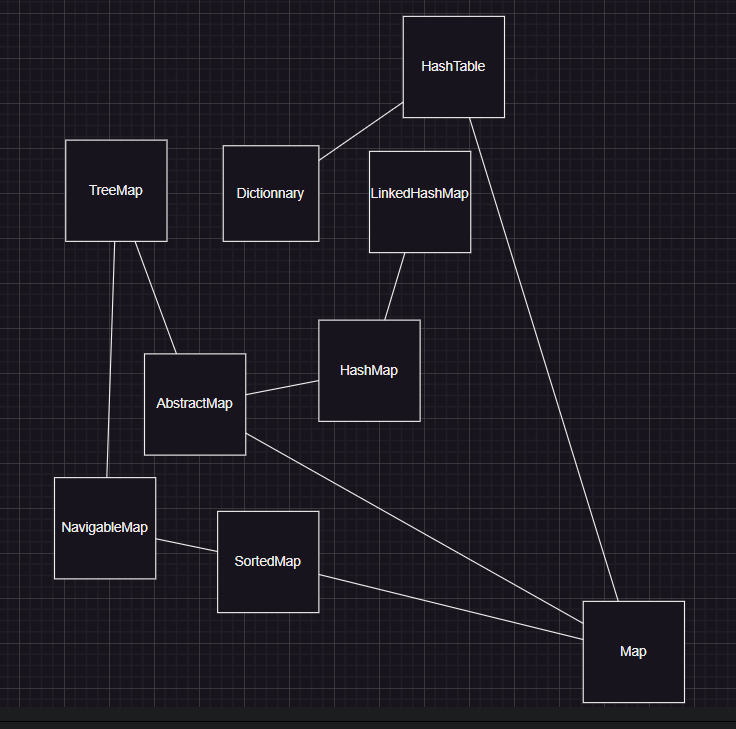
\includegraphics{P6P1Q3.png}\\

\end{enumerate}

\noindent\underline{Part 2}\\
\begin{enumerate}
\item $\subseteq$ is reflexive, because any set is a subset of itself. It is antisymmetric, because if a set is a subset of another set, it the reverse can not be true, unless both sets are the same. The set that is a subset would be fully comprised of some of the elements of the other set, it is impossible that that other set is itself fully comprised of some of the elements of its own subset, unless the two sets are equivalent. This relation is transitive, because for any set B that is a subset of set A, if set C is a subset of set B, then set C is automatically a subset of set A. Therefore, because it is reflexive, antisymmetric and transitive, $\subseteq$is a relation of partial order.
\item $\mathbb{P}V_{2}= \{\{\},\{a\},\{b\},\{c\},\{a,b\},\{a,c\},\{a,b,c\},\{b,c\}\}$. Every set is a subset of itself, so this relation is reflexive. Every set A that is a subset of another set B can not be the subset of that set B if B is not equal to A, so this relation is antisymmetric. This relation is transitive, because if a set B is a subset of a set A, and the set C is a subset of the set B, then set C is automatically a subset of A. Therefore $(\mathbb{P}V_{2}, \subseteq)$ creates a poset.
\item The maximal element is $\{\}$ and the minimal element is $\{a,b,c\}$.\\
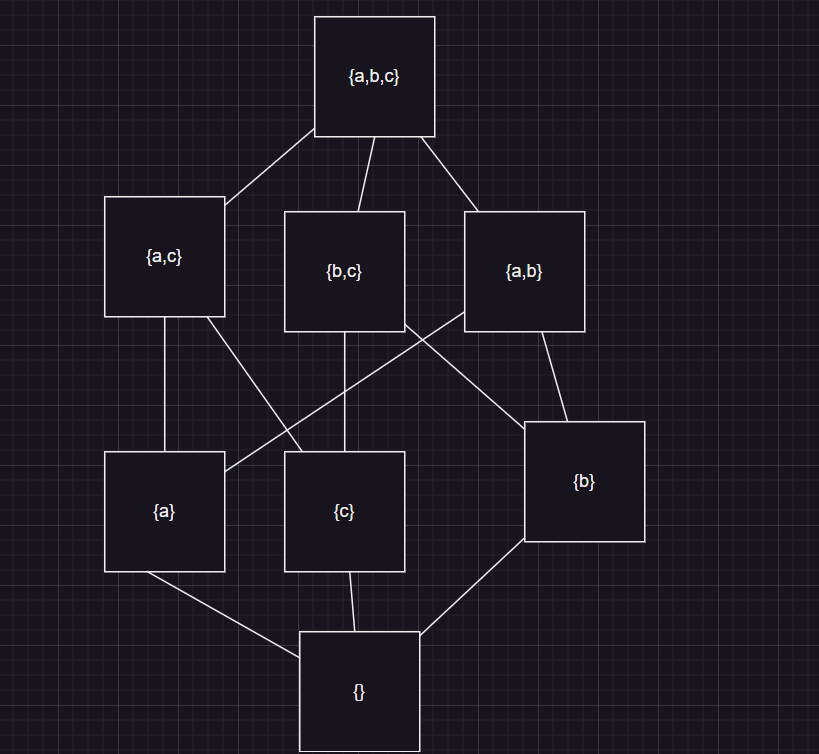
\includegraphics{P6P2Q3.png}\\
\end{enumerate}

\noindent\underline{Part 3}\\
For any element in the domain of map, there is an element in the codomain to which it maps, therefore it is a function. $ \forall x \in domain(map), \exists y \in codomain(map), such that map(x)\mapsto y$. $map$ is a function, but it is a partial function, because it maps only a subset of $(V_{1},R)$.  $(V_{1},R)\not \mapsto (V_{2}, \subseteq)$. $map$ is not an injective function, because {a,b,c} is mapped to by more than one element in the domain. $\exists a,b(a\not {{=}}b\mapsto map(a){{=}}map(b))$. This function is surjective, because every element in the codomain of map is mapped to by at least one element from the domain. $b \in codomain(map), a \in domain(map), map(a)=b, \forall b\exists a(map(a){{=}}b)$. Since it is not injective, map is not bijective.  $\exists a,b(a\not {{=}}b\mapsto map(a){{=}}map(b))$. $map$ is not order preserving because $ AbstractMap \succ TreeMap$, but $map(AbstractMap) \not \succ\ map(TreeMap)$. $\exists x \succ y, map(x) \not \succ mapy(y)$. It is neither order reflecting, because $\varnothing \succ \{c\}$, but $TreeMap \not \succ AbstractMap$. $\exists map(x) \succ map(y), x \not \succ y$. $map$ is not order preserving nor order reflexing, so it can not be order embedding. $\exists map(x) \succ map(y), x \not \succ y$ and $\exists x \succ y, map(x) \not \succ mapy(y)$. $map$ is not order embedding, so it can not be isomorphic. $\exists map(x) \succ map(y), x \not \succ y$ and $\exists x \succ y, map(x) \not \succ mapy(y)$.
\\
\noindent ---------- Remove everything after and including this line after project is completed.
\begin{enumerate}
\item Here is some code in Prolog
\begin{verbatim}
member(X, [X|_]).
member(X, [_|T]) :- member(X, T).
\end{verbatim}


\item LTL formulas:

\begin{enumerate}
	
	\item $\Box \phi \rightarrow \Diamond \psi $
	
	\noindent If $\phi$ is an invariant, then $\psi$ becomes true eventually.
	
	\item $\Box \phi \rightarrow \bigcirc \Box \Diamond \psi$
	
	\noindent If $\phi$ is an invariant, the $\psi$ will be true infinitely often, starting 	
	from the next moment.
	
	\item $(\phi \wedge \bigcirc \psi) \rightarrow \Diamond \Box \tau$	
	
	\noindent If $phi$ is true at time = $i$ and $\psi$ is true at time = $i + 1$,
	then eventually $\tau$ becomes true and stays true.
	
	\item $\Box (( \psi \wedge \bigcirc \chi) \rightarrow \bigcirc \tau)$
	
	\noindent It is always the case that if $\psi$ is true at time = $i$ and if $\chi$ is 	 
	true at time = $i + 1$, then $\tau$ is true at time = $i + 1.$
	
	\item $ (\chi \wedge \bigcirc \omega) \rightarrow \bigcirc^{2} ( \phi ~\mathcal{U}~ \psi )$
	
	\noindent If $\chi$ is true at time = $i$ and if $\omega$ is true at time = $i + 1$,
	then at time  = $i + 2$ $\phi$ becomes true and stays true until $\psi$ becomes 
	true.
	
	\item $( \phi \oplus \psi ) \rightarrow \Box \omega $
	
	\noindent If one of $\phi$ or $\psi$ are true at time = $i$, then $\omega$ becomes at
	invariant at time = $i.$	
	
	
\end{enumerate}


\item The behavior of a program is expressed by the following temporal formula:

\[
\Box	\begin{bmatrix}
	
	1.~~   \textbf{start} \rightarrow \neg a \vee \neg b  \\
	\ \\
	2.~~   \textbf{start} \rightarrow c\\
	\ \\    
	3.~~   b \wedge c \rightarrow \bigcirc^{2} (d \oplus e)\\
	\ \\    
	4.~~   a \vee c \rightarrow \bigcirc (k~\mathcal{R}~g)\\
	\ \\    
	5.~~   (d \vee e) \rightarrow \bigcirc^{2} k\\
	\ \\    
	6.~~   c \rightarrow (h ~\mathcal{W}~ (e \wedge g))\\
	\ \\    
	7.~~   (d \wedge g \wedge h) \rightarrow \bigcirc^{3} m\\
	\ \\
	8.~~   d \rightarrow m~\mathcal{R}~h \\
	\ \\
	9.~~   e \wedge \bigcirc^{2} (k \wedge g) \rightarrow \bigcirc^{2}m \\
	\ \\
	10.~~  (e \wedge g) \rightarrow \bigcirc^{3} c\\
	\ \\
	11.~~  k \wedge m \rightarrow \bigcirc h\\
	\ \\
	12.~~  (e \wedge \bigcirc^{2}k) \rightarrow \bigcirc^{3}b \\
	
\end{bmatrix}
\]





\item Let $B(x)$ denote the subject ``x is a bird'' and $W(x)$ denote the predicate ``x is white.'' Translate the following formal statements into English sentences and attach the corresponding categorical form to each:

\begin{enumerate}
\item $\forall x~(B(x) \rightarrow W(x))$


\item $\forall x~(B(x) \rightarrow \neg W(x))$ 


\item $\exists x~(B(x) \wedge W(x))$ 


\item $\exists x~(B(x) \wedge \neg W(x))$ 
\end{enumerate}

\noindent \underline{Solution}: \\

\begin{enumerate}
\item $\forall x~(B(x) \rightarrow W(x))$ : ``All birds are white.'': (A)
\item $\forall x~(B(x) \rightarrow \neg W(x))$ : ``All birds are non-white.'': (E)
\item $\exists x~(B(x) \wedge W(x))$ : ``Some birds are white.'': (I)
\item $\exists x~(B(x) \wedge \neg W(x))$ : ``There is an non-white bird.'': (O)
\end{enumerate}


\item Describe when the following predicate can be false: $\forall x \exists y P(x, y)$.\\

\noindent \underline{Solution}: The statement can be false when there is an $x$ such that $P(x, y)$ is false for every $y$.



\item Let $P(x, y)$ be the statement ``x asked y out to lunch'' where the domain is all students in class. Express each of the following quantifications in English:

\begin{enumerate}
\item $\exists y \forall x P(x, y)$.\\

\noindent \underline{Solution}: Recall that this reads \textbf{''There in an $y$ that makes $P(x, y)$ true for every $x$.''} There is a student in class who has been asked out to lunch by every student in class.\\

\item $\forall x \exists y P(x, y)$.\\

\noindent \underline{Solution}: Recall that this reads \textbf{``For every $x$ there is a $y$ for which $P(x, y)$ is true.''} Every student in class has asked out to lunch some (at least one) student in class.
\end{enumerate}


\end{enumerate}





\noindent \textbf{An important observation on functions is that we can view them as relations, and as such we can model a function as a set of pairs (tuples)}.

\begin{enumerate}

\item Consider the following relation:

\[ phone : Model \leftrightarrow Brand \]

\noindent where

\[
phone = \\
\{ \\
\hspace{10mm} iPhone7 \mapsto apple,\\
\hspace{10mm} iPhoneX \mapsto apple,\\
\hspace{10mm} galaxyS \mapsto samsung,\\
\hspace{10mm} galaxyA \mapsto samsung,\\
\hspace{10mm} galaxyJ \mapsto samsung,\\
\hspace{10mm} mate20 \mapsto huawei,\\
\hspace{10mm} p20 \mapsto huawei\\
\}
\]

\begin{enumerate}

\item What is the domain of the relation?\\

\noindent $\dom~phone = \{ iPhone7, iPhoneX, galaxyS, galaxyA, galaxyJ, mate20, p20 \}$.


\newpage


\item What is the range of the relation?\\

\noindent $\ran~phone = \{ apple, samsung, huawei \}$.


\ \\


\item What is the result of the expression  $\{ iPhone7, galaxyA \}  \lhd phone$ ?\\


\noindent Domain restriction selects pairs based on their first element. As a result,

\[ \{ iPhone7, galaxyA \}  \lhd phone = \{ iPhone7 \mapsto apple, galaxyA \mapsto samsung \} \]


\noindent Restriction operators are deployed to model database \textit{queries}.


\ \\


\item What is the result of the expression  $phone \rhd \{ apple, samsung \}$ ?\\


\noindent Range restriction selects pairs based on their second element. As a result,

\[ 
phone \rhd \{ apple, samsung \} = \\

\hspace{5mm} \{ \\
\hspace{10mm} iPhone7 \mapsto apple,\\
\hspace{10mm} iPhoneX \mapsto apple,\\
\hspace{10mm} galaxyS \mapsto samsung,\\
\hspace{10mm} galaxyA \mapsto samsung,\\
\hspace{10mm} galaxyJ \mapsto samsung\\
\hspace{5mm} \}
\]


\newpage

\noindent Consider the following Questions to be done in one sequence where we will make permanent modifications to the contents of $phone$:\\


\item What is the result of the expression  $\{ iPhone7, iPhoneX, galaxyA, mate20 \} \ndres phone$ ?\\


\noindent  Domain subtraction removes elements from the domain of the relation:\\


\[
\{ iPhone7, iPhoneX, galaxyA, mate20 \} \ndres phone = \\

\hspace{5mm} \{ \\
\hspace{10mm} galaxyS \mapsto samsung,\\
\hspace{10mm} galaxyJ \mapsto samsung,\\
\hspace{10mm} p20 \mapsto huawei\\
\hspace{5mm} \}

\]

\noindent Note that for a modification to phone, we need to write


\[ phone' = \{ iPhone7, iPhoneX, galaxyA,mate20  \} \ndres phone \]


\noindent which reads as: ``The new value of phone is assigned the value of the evaluation of
the expression on the right-hand-side.''



\item What is the result of the expression  $phone \nrres \{ huawei \}$ ?\\


\noindent  Range subtraction removes elements from the codomain of the relation:\\


\[
phone \nrres \{ huawei\} = \\

\hspace{5mm} \{ \\
\hspace{10mm} galaxyS \mapsto samsung,\\
\hspace{10mm} galaxyJ \mapsto samsung\\
\hspace{5mm} \}

\]


\noindent Assume now that we did

\[ phone' = phone \nrres \{ huawei\} \]


\noindent and as a result, the new value of $phone$ will be

\[
phone = \\

\hspace{5mm} \{ \\
\hspace{10mm} galaxyS \mapsto samsung,\\
\hspace{10mm} galaxyJ \mapsto samsung\\
\hspace{5mm} \}

\]


\ \\


\item What is the result of $phone \oplus \{ iPhoneXSMax \mapsto apple \}$? \\


\noindent Relational overriding can model database updates.

\[
phone \oplus \{ iPhoneXSMax \mapsto apple \} = \\
\hspace{5mm} \{\\
\hspace{10mm} iPhoneXSMax \mapsto apple, \\
\hspace{10mm} galaxyS \mapsto samsung, \\
\hspace{10mm} galaxyJ \mapsto samsung \\
\hspace{5mm} \}
\]

\noindent Note that for a modification to $phone$, we need to write

\[ phone' = phone \oplus \{ iPhoneXSMax \mapsto apple \} \]

\end{enumerate}



\item Consider the sets

\begin{itemize}
\item $Phone = \{ Samsung, Huawei, Apple, Sony, Motorola, HTC \}$, and
\item  $Favorite = \{ Sony, HTC \}$.
\end{itemize}

\noindent Answer the following questions:

\begin{enumerate}

\item How do we interpret the expression $Favorite : \mathbb{P} Phone$?

\item Is $\mathbb{P} Phone$ a legitimate type?

\item What is the nature of the variable in $Favorite : \mathbb{P} Phone$? (i.e. atomic or composite?)

\item Is $Apple \in \mathbb{P} Phone$?

\item Is $\{ Apple \} \in \mathbb{P} Phone$?

\item Is $\{ \{ \} \} \in \mathbb{P} Phone$?

\item Is $\{ \} \in \mathbb{P} Phone$?

\item If we define variable $Favorite : \mathbb{P} Phone$, is $\{ \}$ a legitimate value for variable $Favorite$?

\item Is $Favorite \in \mathbb{P} Phone$?

\item Is $Favorite \subset \mathbb{P} Phone$?

\end{enumerate}

\noindent \underline{Solution}:

\begin{enumerate}

\item How do we interpret the expression $Favorite : \mathbb{P} Phone$? \underline{Answer}: This is  interpreted as ``The variable $Favorite$ can assume any value supported by the powerset of $Phone$.

\item Is $\mathbb{P} Phone$ a legitimate type? \textbf{Yes.}

\item What is the nature of the variable in $Favorite : \mathbb{P} Phone$? \underline{Answer}: Variable $Favorite$ is a \textbf{set}.

\item Is $Apple \in \mathbb{P} Phone$? \textbf{No}.

\item Is $\{ Apple \} \in \mathbb{P} Phone$?  \textbf{Yes}.

\item Is $\{ \{ \} \} \in \mathbb{P} Phone$? \textbf{No}.

\item Is $\{ \} \in \mathbb{P} Phone$? \textbf{Yes}.

\item If we define variable $favorite : \mathbb{P} Phone$, is $\{ \}$ a legitimate value for variable $Favorite$? \textbf{Yes}.

\item Is $Favorite \in \mathbb{P} Phone$? \textbf{Yes}.

\item Is $Favorite \subset \mathbb{P} Phone$? \textbf{No}.

\end{enumerate}










\item Consider the following relation:

\[ laptops : Model \leftrightarrow Brand \]

\noindent where

\[
laptops = \\
\hspace{5mm} \{ \\
\hspace{10mm} legion5 \mapsto lenovo,\\
\hspace{10mm} macbookair \mapsto apple,\\
\hspace{10mm} xps15 \mapsto dell,\\
\hspace{10mm} spectre \mapsto hp,\\
\hspace{10mm} xps13 \mapsto dell,\\
\hspace{10mm} swift3 \mapsto acer,\\
\hspace{10mm} macbookpro \mapsto apple,\\
\hspace{10mm} dragonfly \mapsto hp,\\
\hspace{10mm} envyx360 \mapsto hp\\
\hspace{5mm} \}
\]

\begin{enumerate}

\item What is the domain and the range of the relation?\\

\noindent \underline{Answer}:

\begin{itemize}
\item The domain is defined as:  % \textbf{\underline{Marking:  0.5 pt}}
\[
\dom laptops = \\
\hspace{5mm} \{ \\
\hspace{10mm} legion5,\\
\hspace{10mm} macbookair,\\
\hspace{10mm} xps15,\\
\hspace{10mm} spectre,\\
\hspace{10mm} xps13,\\
\hspace{10mm} swift3,\\
\hspace{10mm} macbookpro,\\
\hspace{10mm} dragonfly,\\
\hspace{10mm} envyx360\\
\hspace{5mm} \}
\]


\item The range is defined as:  $\ran~laptops = \{ lenovo, apple, dell, hp, acer \}$.


\end{itemize}


\item What is the result of the expression

\[ \{ xps15, xps13, swift3, envyx360 \}  \lhd laptops \]

\noindent What is the meaning of operator $\lhd$ and where would you deploy such operator in the context of a database management system?

\newpage

\noindent \underline{Answer}:

\noindent The result is 

\[ \{ xps15, xps13, swift3, envyx360 \}  \lhd laptops = \\
\hspace{5mm} \{ \\
\hspace{10mm} xps15 \mapsto dell,\\
\hspace{10mm} xps13 \mapsto dell,\\
\hspace{10mm} swift3 \mapsto acer,\\
\hspace{10mm} envyx360 \mapsto hp\\
\hspace{5mm} \}
\]

\noindent Domain restriction selects pairs based on their first element. We deploy such operators to model database queries. 


\item What is the result of the expression

\[ laptops \rhd \{ lenovo, hp \} \]

\noindent What is the meaning of operator $\rhd$ and where would you deploy such operator in the context of a database management system?

\noindent \underline{Answer}:

\noindent The result is 


\[ laptops \rhd \{ lenovo, hp \} = \\
\hspace{5mm} \{ \\
\hspace{10mm} legion5 \mapsto lenovo,\\
\hspace{10mm} spectre \mapsto hp,\\
\hspace{10mm} dragonfly \mapsto hp,\\
\hspace{10mm} envyx360 \mapsto hp\\
\hspace{5mm} \}
\]

\noindent Range restriction selects pairs based on their second element. We deploy such operators to model database queries. 


\item What is the result of the expression

\[ \{ legion5, xps15, xps13, dragonfly \} \ndres laptops \]

\noindent What is the meaning of operator $\ndres$ and where would you deploy such operator in the context of a database management system?

\noindent \underline{Answer}:

\noindent \noindent The result is 

\[ \{ legion5, xps15, xps13, dragonfly \} \ndres laptops = \\
\hspace{5mm} \{ \\
\hspace{10mm} macbookair \mapsto apple,\\
\hspace{10mm} spectre \mapsto hp,\\
\hspace{10mm} swift3 \mapsto acer,\\
\hspace{10mm} macbookpro \mapsto apple,\\
\hspace{10mm} envyx360 \mapsto hp\\
\hspace{5mm} \}
\]

\noindent  Domain subtraction removes elements from the domain of the relation. We deploy such operation to model deletion of records. 


\item What is the result of the expression

\[ laptops \nrres \{ apple, dell, hp \} \]

\noindent What is the meaning of operator $\nrres$ and where would you deploy such operator in the context of a database management system?

\newpage

\noindent \underline{Answer}:


\noindent \noindent The result is 

\[
laptops \nrres \{ apple, dell, hp \} = \\
\hspace{5mm} \{ \\
\hspace{10mm} legion5 \mapsto lenovo,\\
\hspace{10mm} swift3 \mapsto acer\\
\hspace{5mm} \}
\]
 
 
\noindent  Range subtraction removes elements from the codomain of the relation. We deploy such operation to model database updates (deletion of records). % \textbf{\underline{Marking:  1.5 pts}}



\item Consider the following expression

\[ laptops \oplus \{ ideapad \mapsto lenovo \} \]


\begin{enumerate}
\item What is the result of the expression?

\item What is the meaning of operator $\oplus$ and where would you deploy such operator in the context of a database management system?

\item Does the result of the expression have a permanent effect on the database (relation)? If not, describe in detail how would you ensure a permanent effect. 

\end{enumerate}

\newpage

\noindent \underline{Answer}:


\begin{enumerate}
\item  The result is 

\[ laptops \oplus \{ ideapad \mapsto lenovo \} = \\
\hspace{5mm} \{ \\
\hspace{10mm} ideapad \mapsto lenovo,\\
\hspace{10mm} legion5 \mapsto lenovo,\\
\hspace{10mm} macbookair \mapsto apple,\\
\hspace{10mm} xps15 \mapsto dell,\\
\hspace{10mm} spectre \mapsto hp,\\
\hspace{10mm} xps13 \mapsto dell,\\
\hspace{10mm} swift3 \mapsto acer,\\
\hspace{10mm} macbookpro \mapsto apple,\\
\hspace{10mm} dragonfly \mapsto hp,\\
\hspace{10mm} envyx360 \mapsto hp\\
\hspace{5mm} \}
\]

\item Relational overriding can model database updates (addition of records).


\item The expression does not have a permanent effect on the database (relation). To ensure a permanent effect on the relation, we need to define an assignment statement

\[ laptops' = laptops \oplus \{ ideapad \mapsto lenovo \} \]

\noindent which reads ``The value of variable (relation) $laptops$ is assigned the result of the expression on the right-hand-side of the assignment statement.''

\end{enumerate}
\end{enumerate}

\newpage

\item You can produce a figure using any drawing package and save it as an image e.g. \texttt{.png}.  The image file can then be embedded in your \texttt{.tex} document as follows:

\begin{figure}[h!]
	\centering
	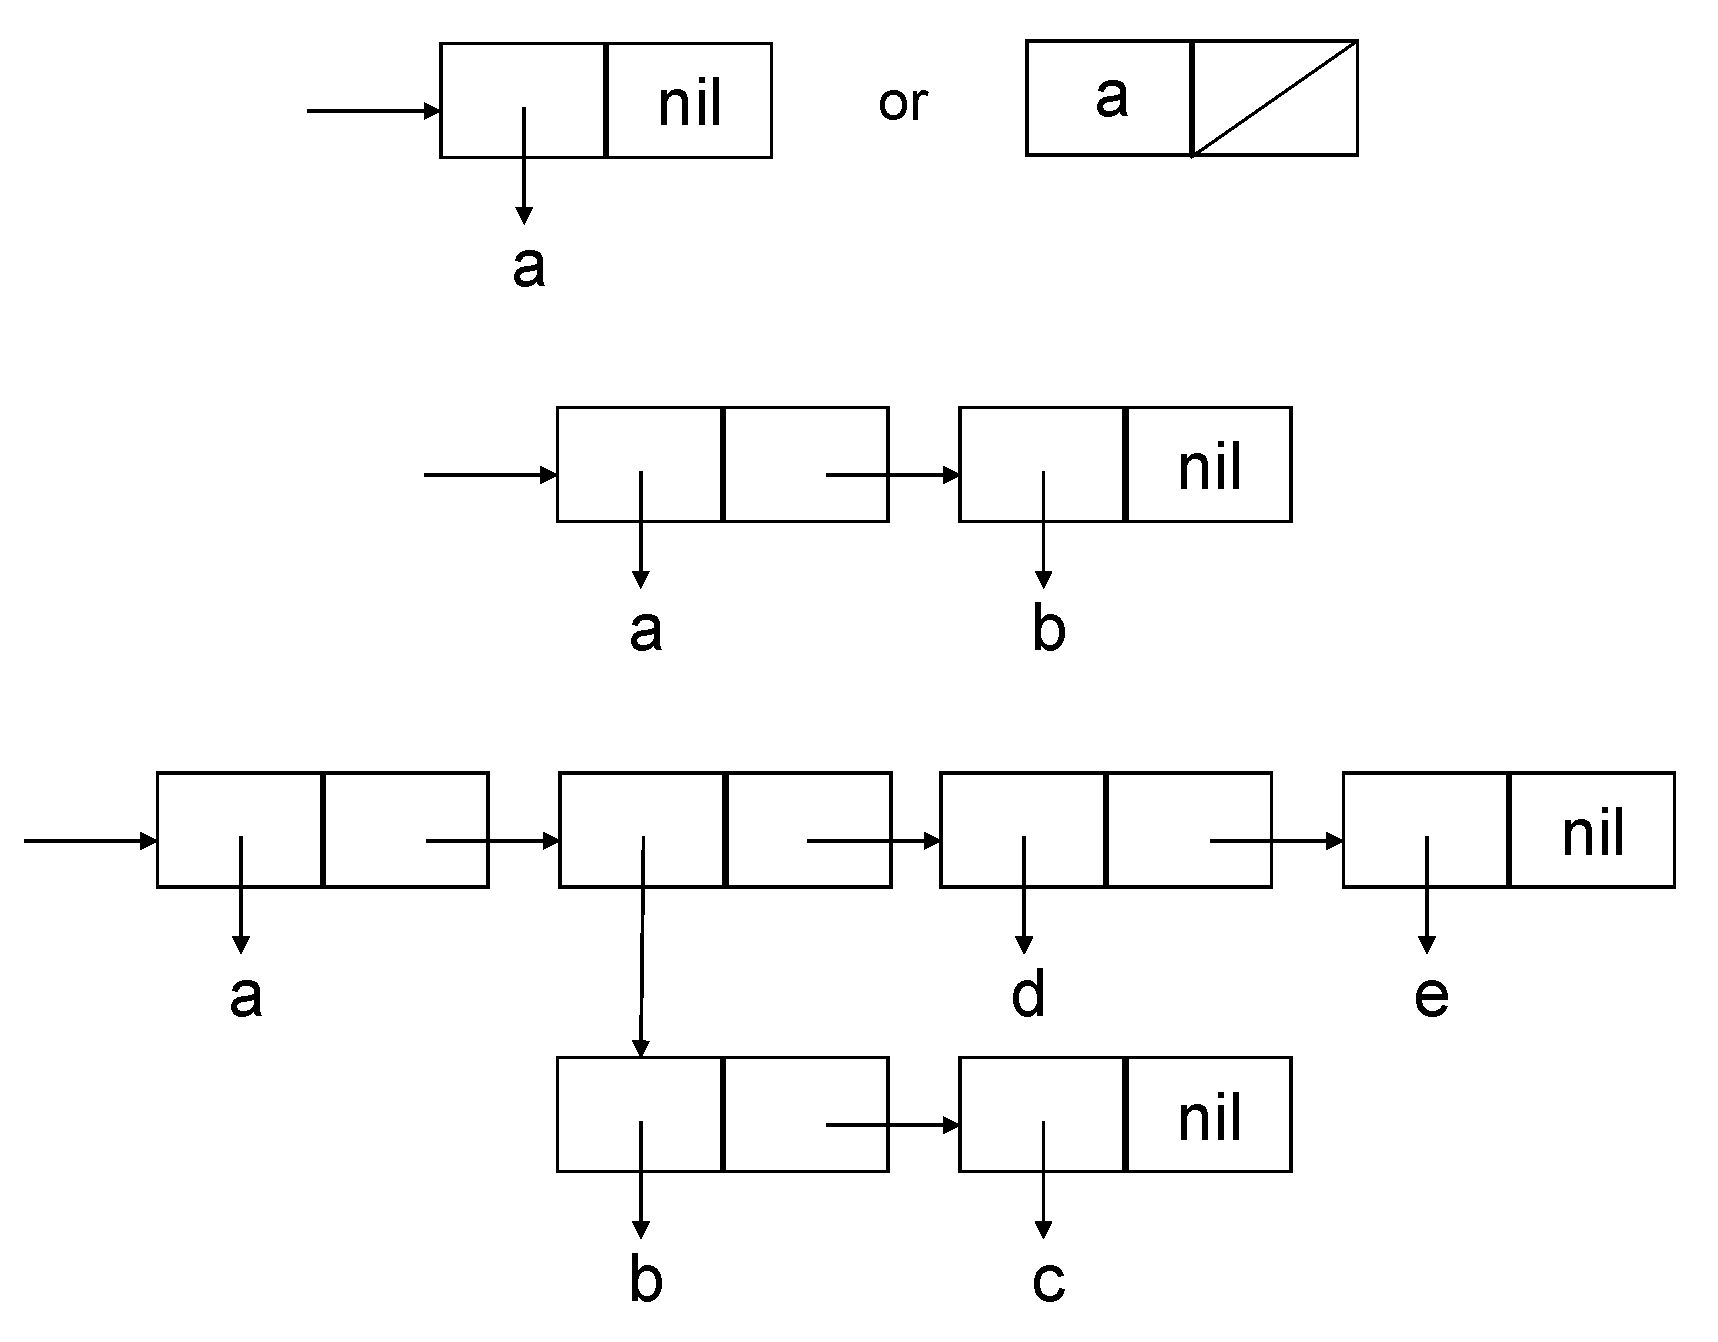
\includegraphics[width=0.6\textwidth]{lists.png}
\end{figure}











\end{enumerate}

\end{spacing}

\end{document}
